
%(BEGIN_QUESTION)
% Copyright 2007, Tony R. Kuphaldt, released under the Creative Commons Attribution License (v 1.0)
% This means you may do almost anything with this work of mine, so long as you give me proper credit

Tegn responsen til en regulator med proporsjonal + integralvirkning, med proporsjonalbånd 50\% og integralkonstant 1.25 minutter per repetisjon, for følgende inngangsbetingelser. Anta at regulatoren er {\it reversvirkende}:

$$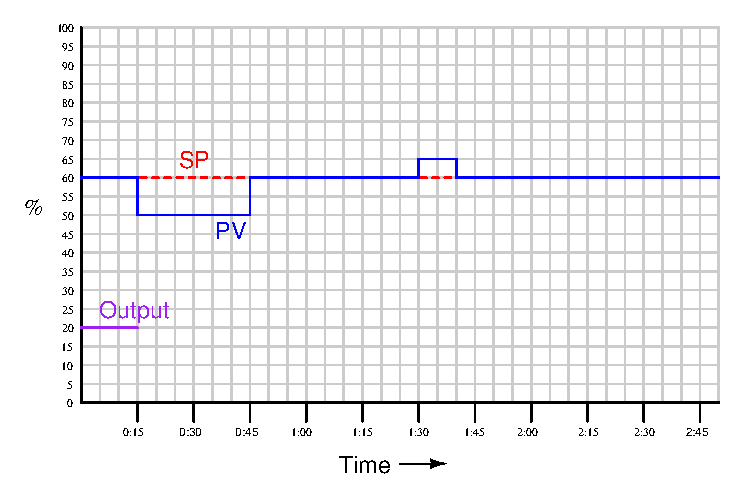
\includegraphics[width=15.5cm]{i01604x01.eps}$$

Tidsskalaen i diagrammet er minutter:sekunder, og PI-algoritmen er som følger:

$$m = K_p \left( e + {1 \over \tau_i} \int e \> dt \right) + b$$

\noindent
Der,

$m$ = regulatorutgang (manipulert variabel)

$K_p$ = forsterkning

$e$ = avvikssignal (SP$-$PV)

$\tau_i$ = integraltidskonstant

$b$ = bias

\vskip 10pt

\underbar{file i01604}
%(END_QUESTION)





%(BEGIN_ANSWER)

$$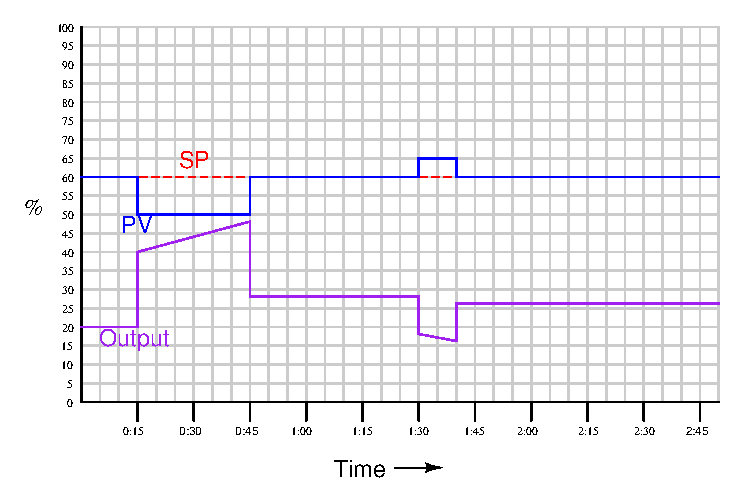
\includegraphics[width=15.5cm]{i01604x02.eps}$$

På PV-trinnendringen på -10\% responderer regulatoren umiddelbart med et utgangstrinn på 20\% (proporsjonalbånd 50\% tilsvarer forsterkning 2), og utgangen går fra opprinnelig 20\% til 40\%. Deretter får det vedvarende avviket på -10\% integralvirkningen til å rampe utgangssignalet med 16\% per minutt (20\% proporsjonalrespons multiplisert med 0.8 repetisjoner per minutt). Siden avviket på -10\% mellom PV og SP bare varer i 30 sekunder (mellom 0:15 og 0:45), rekker utgangssignalet bare å rampe 8\%, slik at utgangen blir 48\% ved slutten av første avviksperiode.

Når PV så returnerer til SP (et +10\% trinn), hopper utgangen ned 20\%, og blir liggende 8\% høyere enn startverdien (28\%, fra opprinnelig 20\%).

Når neste PV-trinnendring kommer ved 1:30, gir trinnet på +5\% oppover et umiddelbart utgangstrinn på -10\% på grunn av proporsjonalvirkning, slik at utgangen blir 18\%. Integralvirkningen, med hastighet 0.8 repetisjoner per minutt, tar proporsjonalresponsen på -10\% og gir en utgangsstigning på -8\% per minutt. Siden denne trinnperioden bare varer i 10 sekunder (1:30 til 1:40), blir akkumulert utgangsendring fra integral -1.333\%, og utgangen faller til en lavverdi på 16.67\%. Når PV returnerer til SP (hopper ned 5\%), hopper utgangen opp 10\%, slik at endelig utgangsverdi blir 26.67\% ut resten av grafen.

%(END_ANSWER)





%(BEGIN_NOTES)


%INDEX% Control, proportional + integral: graphing controller response

%(END_NOTES)
